%!TEX root=../document.tex

\section{Ergebnis}
\label{sec:Ergebnis}

Folgende Punkte wurden bearbeitet:


\begin{itemize}
	\item Allgemein
	\item CherryPy und andere angewendeten Technologien
	\item Vorgehensweise
	\item Aufgetretene Probleme	
	\item Ergebnis
\end{itemize}


\subsection{Allgemein}

Wir haben uns für CherryPy entschieden und für einen Anwendungsfall, der schnell zu implementieren und eine niedrige Komplexität aufweist. Das ist laut CherryPy einer der häufigsten Anwendungsfälle für CherryPy. Ein weiterer wichtiger Vorteil ist, dass CherryPy auf OOP ausgelegt ist und lässt sich dadurch zusätzlich leichter schreiben und verstehen.

Wir haben eine Webseite mit CRUD-Funktionen erstellt mit denen man Benutzer verwalten kann. 
Dazu haben wir in der Datenbank eine Tabelle angelegt die wie folgt ausschaut
\begin{figure}[!h]
\centering
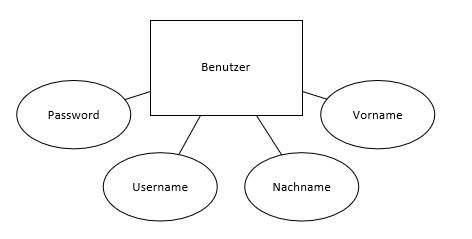
\includegraphics[width=0.5\linewidth]{images/db}
\caption{Aufbau von Benutzer}
\label{fig:Benutzeraufbau}
\end{figure}


Das Einsteigen in CherryPy ist mit Abstand einer der größten Vorteil, den mit wenigen Zeilen lässt sich eine Webseite erstellen und bereitstellen.
\begin{lstlisting}[language=Python]
import cherrypy

class HelloWorld(object):
@cherrypy.expose
def index(self):
return "Hello World!"

cherrypy.quickstart(HelloWorld())
\end{lstlisting}

Mit diesen Zeilen ist eine Webseite erstellt und funktionsfähig.

Insgesamt beläuft sich der Arbeitsaufwand auf ungefähr \textbf{10 Stunden}.

\subsection{CherryPy und andere angewendeten Technologien}

CherryPy ist ein Non-Full-Stack-Framework und bietet mit einer sehr einfachen Verfahren einen Webserver an, der mit wenigen Befehlen gestartet und mit Inhalt gefüllt werden kann.

Weiters haben wir für unsere Persistierung die eingebaute Schnittstelle von Python zu SQLite verwendet. Dieses Schnittstelle ermöglicht es mit wenigen Befehlen eine simple Datenbank zu betreiben. Allerdings hatten wir auch einigen Probleme mit der Datenbank auf die wir später noch genauer eingehen.

Um die Webseite mit der CherryPy-Rückgaben zu verbinden, haben wir jQuery verwendet. 

Zusätzlich haben wir, um der Webseite ein sprechenden Design zu geben, CSS und Bootstrap verwendet. 


\subsection{Umsetzung}

Die Übung ist in 2 Bereiche aufzuteilen, den Server Teil, dieser kümmert sich um das Speichern und Lesen aus der Datenbank, diese Aufgabe wurde mittels den Python WebFramework CherryPy umgesetzt. Der Client Teil kümmert sich hingegen um die Darstellung sowie um die Eingaben, dies wurde mittels HTML, CSS und JavaScript umgesetzt.

\subsubsection{CherryPy}

Als erstes wurde eine Klasse CRUD erstellt, diese wird aufgerufen sobald man auf localhost mit der entsprechenden Port Nummer zugreift. Die Klasse öffnet die index.html Datei und sendet den Inhalt an den Browser zurück.

\begin{lstlisting}[language=Python, caption=Klasse zur Darstellung der Index.html]
class CRUD(object):
@cherrypy.expose
def index(self):
return open('index.html')
\end{lstlisting}

Nun wurde eine Klasse erstellt, welche auf die HTML Befehle reagiert, dies sind GET, POST, PUT, ... . In unserem Fall haben wir nur POST verwendet mit 2 Parameter. Der erste Parameter param gibt an welche Aktion wir durchführen wollen, der zweite Parameter input gibt liefert zusätzliche Informationen, wie zum Beispiel eingeben Werte.

\begin{lstlisting}[language=Python, caption=Klasse zur verwaltung der HTML Befehle]
@cherrypy.expose
class CRUDWebService(object):

@cherrypy.tools.accept(media='text/plain')
def POST(self, param, input):
\end{lstlisting}
\clearpage
Wird ein read als Parameter gesendet, erwartet sich der Client alle Benutzer. Aus diesem Grund werden alle Benutzer aus der Datenbank ausgelesen und eine HTML Tabelle erstellt. Diese wird dann als HTML Response zum Client zurückgesendet und dargestellt.

\begin{lstlisting}[language=Python, caption=Auslesen aller Benutzer aus der Datenbank]
if param == "read":
with sqlite3.connect(DB_STRING) as c:
r = c.execute("SELECT * FROM benutzer")
response = "<table width='100%' class='table table-striped 		table-bordered'" \
"cellspacing='0'><tr><td>Nr</td><td>Vorname</td><td>Nachname</td>" \
"<td>Username</td></tr>"
while True:
row = r.fetchone()
if row is None:
break
response += "<tr><td>" + str(row[0]) + "</td><td>" + row[1] + "</td><td>" + row[2] + "</td><td>" \
+ row[3] + "</td></tr>"
response += "</table>"
return response
\end{lstlisting}

Auf den Parameter update reagiert das Programm sehr ähnlich, einziger Unterschied ist, dass die Benutzer in einer Tabelle zurückgeliefert werden, die bei jedem Benutzer einen Button zum Bearbeiten hat. Außerdem müsste hier ein kurzes sleep eingebaut werden, da update gleich nach einer Datenbank ändern die neuen Benutzer ausliest, dadurch konnte es passieren das beim Auslesen noch nicht die neuen Werte dabei waren.

\begin{lstlisting}[language=Python, caption=Auslesen aller Benutzer aus der Datenbank und bearbeitbar zurückliefern]
if param == "update":
sleep(0.05)
with sqlite3.connect(DB_STRING) as c:
r = c.execute("SELECT * FROM benutzer")
response = "<table width='100%' class='table table-striped table-bordered'" \
"cellspacing='0'><tr><td>Nr</td><td>Vorname</td><td>Nachname</td>" \
"<td>Username</td><td>Aendern</td></tr>"
while True:
row = r.fetchone()
if row is None:
break
response += "<tr><td>" + str(row[0]) + "</td><td>" + row[1] + "</td><td>" + row[2] + "</td><td>" \
+ row[3] + "</td><td> <button onClick='updateBenutzer(" + str(row[0]) + ")'>Aendern" \
"</button></td></tr>"
response += '</table>'
return response
\end{lstlisting}


\subsection{Aufgetretene Probleme}

\subsubsection{Tabelle nicht gefunden}
Die häufigste Fehlermeldung dieser Art war: $ no\,such\,table:\,benutzer $ 

Diesen Fehler konnten wir auf keine genaue Stelle eingrenzen, da dieser Fehler zufällig beim Starten des Server hin und wieder aufgetretten ist. 

Gelöst haben wir diesen Fehler dann durch das Sicherstellen, dass die Tabelle noch existiert und wenn nicht die Tabelle neu erstellt und mit Standarddatensätzen wieder befüllt wird.

\subsubsection{Datensatz nicht richtig abgespeichert}
Ein Fehler, der leicht zu lösen war, war: $ no\,such\,attribute:\,zuba $ 

Hierbei hat es sich um eine INSERT Anweisung gehandelt, die eine syntaktisch falschen Aufbau hatte, den wir allerdings erst sehr spät bemerkt haben. 

Gelöst haben wird dies, indem wir die Zusammensetzung der Anweisung neu geschrieben haben und explizit die Reihenfolge der Attribute angegeben haben.



%\subsubsection{JS Funktionen nicht aufrufbar}$ function\,showuser\,not\,found $ 

%\subsubsection{Aufrufprobleme}Delete konnte Daten nicht anzeigen, wenn davor Anzeigen aufgerufen wurde


\subsection{Ergebnis}

Das Ergebnis der Übung ist eine Webseite, die die CRUD Funktionen bereitstellt, um Benutzer zu verwalten.

CREATE:
\begin{figure}[!h]
\centering
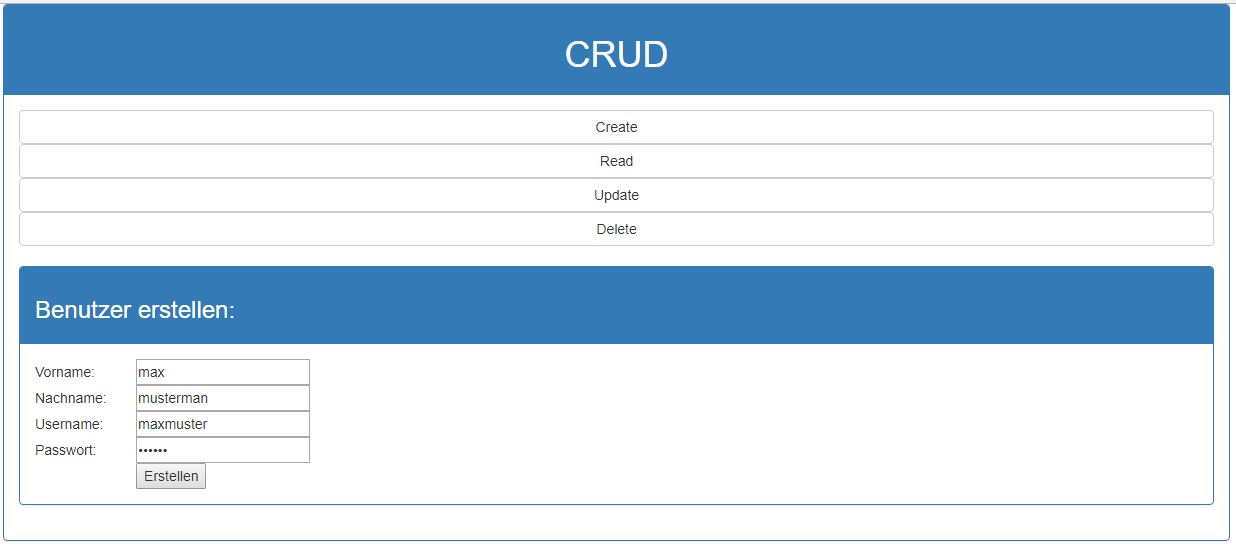
\includegraphics[width=1\linewidth]{images/create}
\caption{CREATE Funktion}
\label{fig:create}
\end{figure}
\clearpage
READ:
\begin{figure}[!h]
\centering
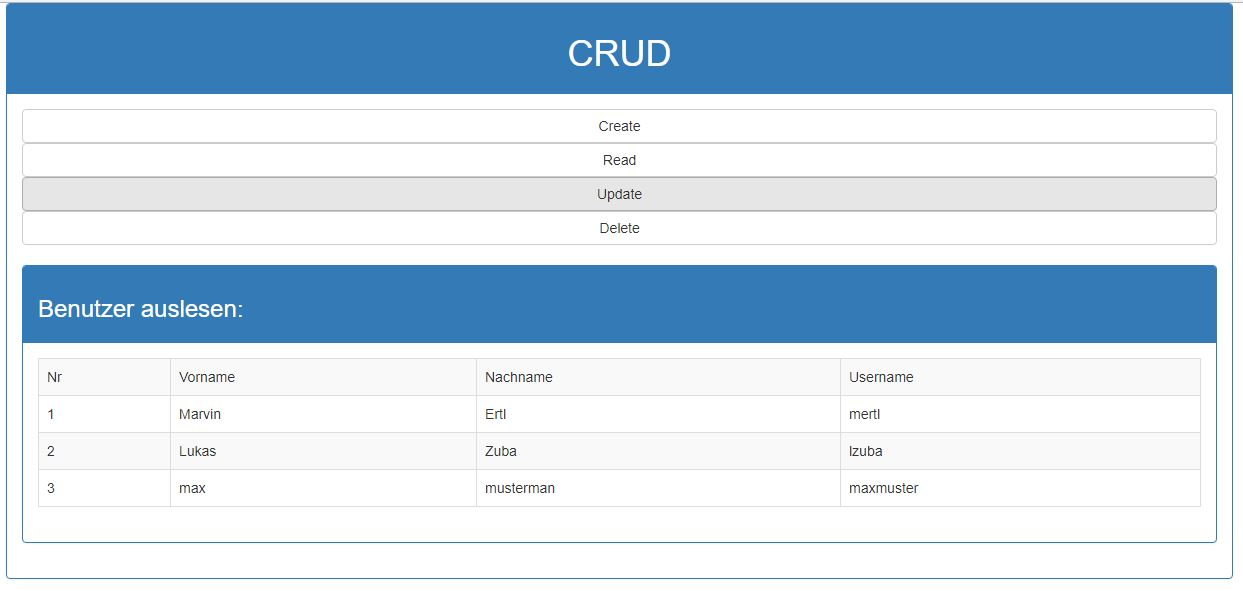
\includegraphics[width=0.9\linewidth]{images/read}
\caption{READ Funktion}
\label{fig:read}
\end{figure}

UPDATE:
\begin{figure}[!h]
\centering
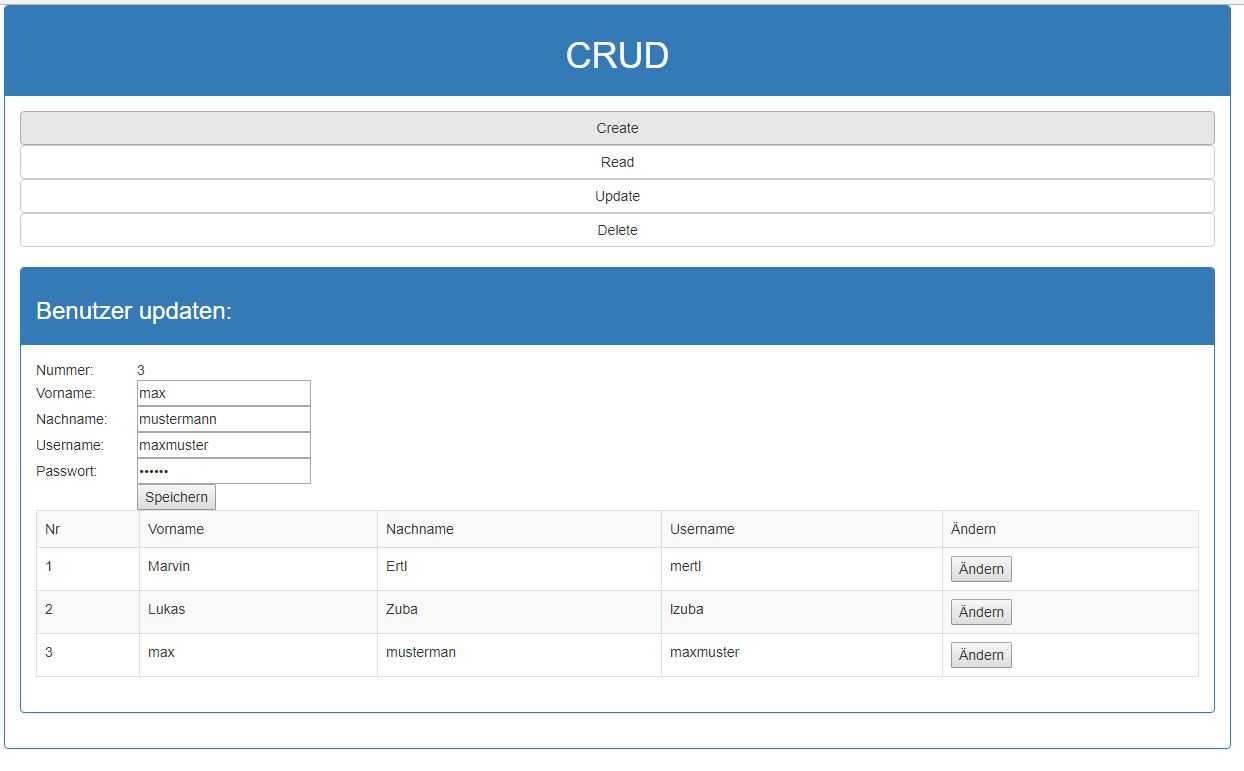
\includegraphics[width=0.9\linewidth]{images/update}
\caption{UPDATE Funktion}
\label{fig:update}
\end{figure}
\clearpage
DELETE:
\begin{figure}[!h]
\centering
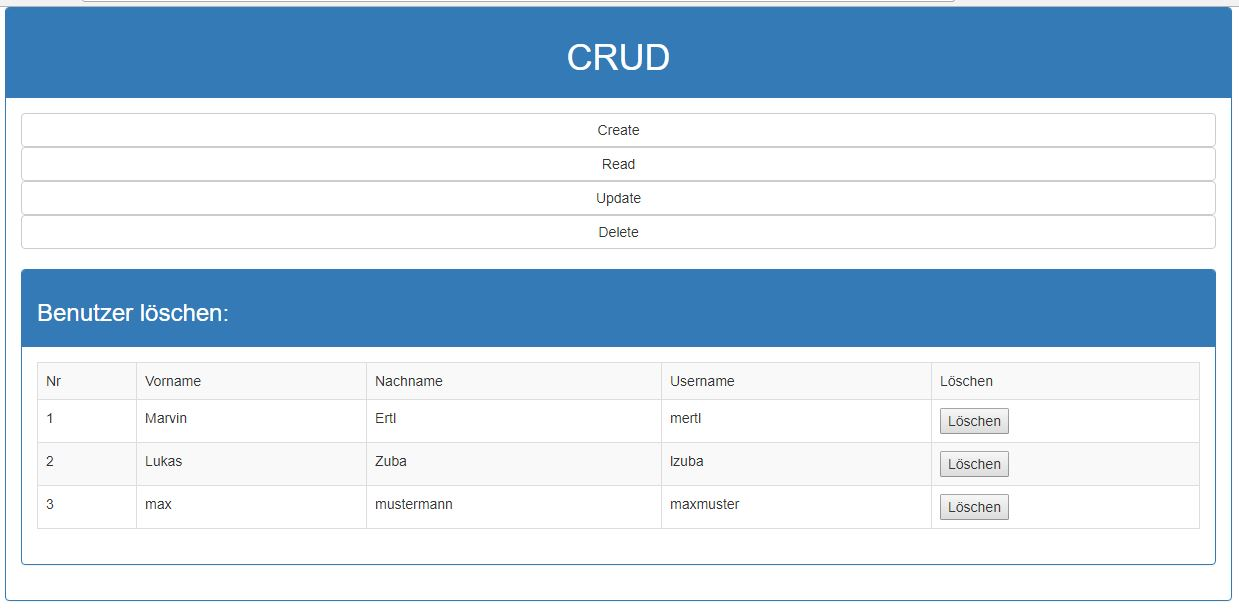
\includegraphics[width=1\linewidth]{images/delete}
\caption{DELETE Funktion}
\label{fig:delete}
\end{figure}

\begin{figure}[!h]
\centering
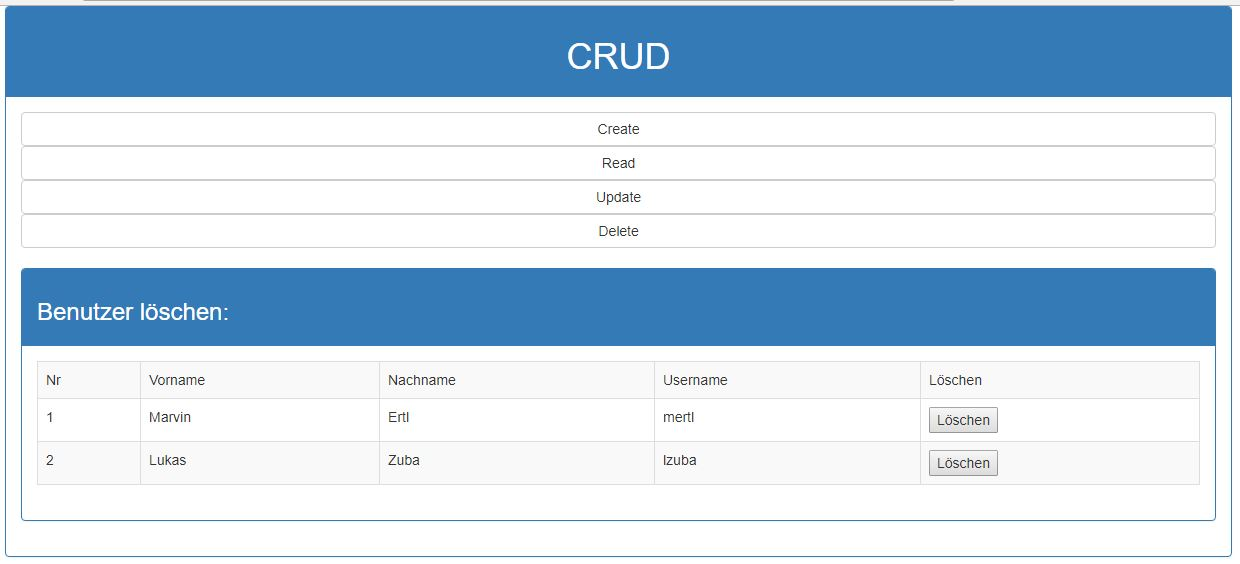
\includegraphics[width=1\linewidth]{images/delete_after}
\caption{DELETE nach dem Löschen von Max Mustermann}
\label{fig:deleteafter}
\end{figure}

